% arara: lualatex: {options: ['--output-directory=docs_saida']}
%% arara: lualatex: {options: ['--output-directory=docs_saida']}

% classe com as customizações -------------------------------------------------
\documentclass{minicursoUFRB}

%==============================================================================
% Início do Documento 
%------------------------------------------------------------------------------
\begin{document}
%
  \capa
%
  \thispagestyle{empty}
  \tableofcontents
%
	\flushbottom
	\newpage
%
	%==============================================================================
% Introdução ao texto
%==============================================================================
\thispagestyle{empty}

\section*{Bate-papo Inicial}

\begin{marginfigure}
  \centering
  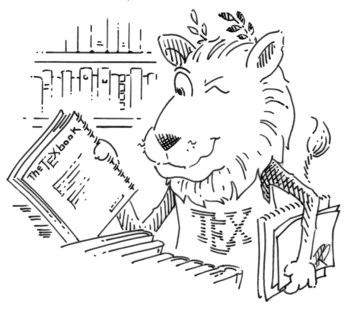
\includegraphics[width = \linewidth]{ctan_lion_350x350}
\end{marginfigure}

Se você optou por ler esse material, vá até o fim!
O \LaTeX\ pode ser para você uma ferramenta extremamente agradável para produção
tipográfica, a nível profissional, de suas futuras notas de aula; monografias,
dissetações ou teses; listas de atividades; partituras; marcações no xadrez; etc.

Não pretendo abordar muita coisa, confesso.

Fui incumbido de ministrar, em pouco mais de 3\unit{\hour}, uma introdução ao 
\LaTeX.

\begin{codigo}{Exemplo de preâmbulo}{\lapis}
% arara: lualatex: {options: ['--output-directory=docs_saida']}

% classe do documento -------------------------------------------------------
\documentclass[12pt]{article}

% pacotes carregados --------------------------------------------------------
\usepackage{mathtools, amsfonts, amsthm}

% configurações do título ---------------------------------------------------
\title{\textbf{Título}}
\author{Ícaro Vidal Freire}
\date{\today}

%============================================================================
% Início do Documento
%----------------------------------------------------------------------------
\begin{document}
%
  \maketitle % produz a saída do título
%
\begin{abstract}
  Pequeno resumo.
\end{abstract}
%
\section{Primeira Seção}

Olá \LaTeX!
%---------------------------------------------------------------------------- 
\end{document}
%============================================================================
\end{codigo}

%------------------------------------------------------------------------------
\newpage
%
  \pagestyle{fancynotes}
%
	\part{Introduction}	
	\section{Primeiro Teste }
	\lipsum[1]
	\section{Segundo Teste}
	\lipsum[2-3]
  %\section{Motivation}\label{sec:motivation}
\begin{margintable}\vspace{.8in}\footnotesize
  \begin{tabularx}{\marginparwidth}{|X}
  Section~\ref{sec:motivation}. Motivation\\
  Section~\ref{sec:reqpackages}. Required Packages\\
  Section~\ref{sec:license}. Margins\\
  \end{tabularx}
\end{margintable}
During my year as a Part III student at Cambridge, I realized that my theoretical physics professors, namely David Tong and David Skinner, would use the \texttt{jhep} format to typeset the notes for their classes. As the year went on, I started typesetting my personal notes during class and realized that the \texttt{jhep} format, while great for publications and lecture notes in general, was lacking a few small but useful features.

I came across James P. Sethna's wonderful text on statistical mechanics, published by the Oxford University Press, and loved the formatting of the OUP. Sadly the OUP does not have a publicly released LaTeX .sty file for their content, and while the Memoir class and the Tufte style packages provide extensive functionality, I needed something slightly different and a package that was more readily modifiable. Enter \textit{NotesTeX}.

The result of this year long work, from 2016-2017, is the package now known as \textit{NotesTeX.} The purpose of this package was to consolidate all these changes that I slowly incorporated into the original \texttt{jhep} format, and to provide stable support for commonly used physics and mathematics environments. I sincerely hope that you enjoy the package!


\section{Required Packages}\label{sec:reqpackages}
For \textit{NotesTeX,} the following packages are required
\begin{center}
  \texttt{marginnote, sidenotes, fancyhdr, titlesec, geometry, and tcolorbox.}
\end{center}
The roles of each of these packages will be discussed in Part~\ref{Part:Modification}. However, for a brief summary, the \texttt{marginnote}, \texttt{sidenote}, \texttt{titlesec}, and \texttt{tcolorbox} packages are used in creating the \texttt{$\backslash$part} environment, the package \texttt{geometry} is used globally to set the page width, page height, and margin width, and finally, \texttt{fancyhdr}, which is overridden on the title page, the contents page, and the \texttt{$\backslash$part} page, sets the header for the body.

\section{License}\label{sec:license}
Aditya Dhumuntarao does not own the copyright to the original package, \texttt{jheppub.sty}. All modification have been approved by the Jhep Editorial committee, and permission has been attributed to Aditya to distribute freely the modified version of \texttt{jheppub.sty}, known as \texttt{NotesTeX.sty}.

This work may be distributed and/or modified under the conditions of the LaTeX Project Public License, either version 1.3 of this license or (at your option) any later version. The latest version of this license is found \href{http://www.latex-project.org/lppl.txt}{here}, and version 1.3 or later is part of all distributions of LaTeX version 2005/12/01 or later. The current maintainer of this work is Aditya Dhumuntarao.\footnote{Please contact me at my email if you have any questions or comments.}

\newpage
%
	%\part{Modifications}\label{Part:Modification}
  %\section{Features}\label{sec:Features}
\begin{margintable}\vspace{1.4in}\footnotesize
  \begin{tabularx}{\marginparwidth}{|X}
  Section~\ref{sec:Features}. Features\\
  Section~\ref{sec:incpackage}. Included Packages\\
  Section~\ref{Sec:Margins}. Margins\\
  Section~\ref{sec:shortcuts}.  Shortcuts\\
  Section~\ref{Sub:Special}. \texttt{amsthm} Environments\\
  Section~\ref{sec:part}. Part Environment\\
  Section~\ref{Sec: Fullpage}. Fullpage Environment\\
  \end{tabularx}
  \caption{Contents for \textsc{Part II}}
\end{margintable}
While \textit{NotesTeX}\footnote{Affectionately called \textit{NoTeX}.} inherits most of the \texttt{jhep} formatting for sections, subsections, subsubsections, title page, contents page, and bibliography presets, there are significant departures from the original format and underlying features. The central focus of this package was to expand the use of the margin in order to include; simple marginnotes, numbered side--notes, marginfigures, and margintables. The secondary motivation was to include a list of preloaded packages that any physics or mathematics students would require while type--setting notes. Lastly, there are a few stylistic improvements that allow for better readability.\\

\noindent \textit{NotesTeX} includes the following:
\begin{enumerate}
  \item Several mathematics and physics packages.
  \item Margins and margin environments for tables, figures, and asides.
  \item \TeX\ shortcuts for various math scripts namely vector bold math, \texttt{mathbb}, \texttt{mathfrak}, and \texttt{mathcal}.
  \item \texttt{amsthm} integrations and special environments for theorems, lemmas, proofs, definitions, examples, and remarks.\
  \item Stylized support for the \texttt{part} environment.
  \item A fullpage environment that spans across the text width and the margin for longer equations and horizontal figures.
\end{enumerate}
Each of these will be discussed in the following subsections.

\section{Included Packages} % (fold)
\label{sec:incpackage}
Additional package are listed right under the required packages in \texttt{NotesTeX.sty}. These are divided into font styling packages and mathematical and physics related packages. The list of packages are also reiterated here and their links are in the sidenotes.
\begin{verbatim}
  \usepackage[T1]{fontenc}                            % Font Styling
  \usepackage{lmodern,mathrsfs}
\end{verbatim}
\begin{margintable}\footnotesize 
  \begin{tabularx}{\marginparwidth}{|X}
    \href{https://www.ctan.org/pkg/fontenc}{fontenc}\\
    \href{https://www.ctan.org/pkg/mathrsfs}{mathrsfs}\\
    \href{https://www.ctan.org/pkg/enumitem}{enumitem}\\
    \href{https://www.ctan.org/pkg/mathtools}{mathtools}\\
    \href{https://www.ctan.org/pkg/amsfonts}{amsfonts}\\
    \href{https://www.ctan.org/pkg/amsthm}{amsthm}\\
    \href{https://www.ctan.org/pkg/bm}{bm}\\
    \href{https://www.ctan.org/pkg/array}{array}\\
    \href{https://www.ctan.org/pkg/tabularx}{tabularx}\\
    \href{https://www.ctan.org/pkg/booktabs}{booktabs}\\
    \href{https://www.ctan.org/pkg/graphicx}{graphicx}\\
    \href{https://www.ctan.org/pkg/float}{float}\\
    \href{https://www.ctan.org/pkg/caption}{caption}\\
    \href{https://www.ctan.org/pkg/setspace}{setspace}\\
    \href{https://www.ctan.org/pkg/multicol}{multicol}\\
    \href{https://www.ctan.org/topic/pgf-tikz}{tikz}\\
    \href{https://www.ctan.org/pkg/physics}{physics}\\
    \href{https://www.ctan.org/pkg/cancel}{cancel}
  \end{tabularx}
  \caption{Links}
\end{margintable}
\begin{verbatim}
  \usepackage[shortlabels]{enumitem}                  % Enumitem Options
  \usepackage{mathtools,amssymb,amsfonts,amsthm,bm}   % Math Presets
  \usepackage{array,tabularx,booktabs}                % Table Presets
  \usepackage{graphicx,wrapfig,float,caption}         % Figure Presets
  \usepackage{setspace,multicol}                      % Text Presets
  \usepackage{tikz,physics,cancel}                    % Physics Presets
\end{verbatim}

% section prepackage (end)


\newpage


\section{Margins}\label{Sec:Margins}%
\textit{NotesTeX} inherits all the margin commands that are used by \texttt{sidenote} and \texttt{marginnote}, and two additional pre-configured commands known as \texttt{$\backslash$mn} and \texttt{$\backslash$sn}. The relevant commands, and the packages they belong to, are
\begin{center}
  \begin{multicols}{2}
  \noindent\texttt{$\backslash$marginfigure~[sidenote]\\
  $\backslash$sidenote~[sidenote]\\
  $\backslash$marginnote~[marginnote]\\
  $\backslash$margintable~[sidenote]\\
  $\backslash$sn~[NotesTeX]\\
  $\backslash$mn~[NotesTeX]\\
  }
\end{multicols}
\end{center}
The implementation of each of these is as follows.
\begin{enumerate}
  \item \texttt{Marginnote:} This is how a \texttt{$\backslash$marginnote\{...\}} behaves.\marginnote{Not numbered, 10pt.}
  \item \texttt{Mn:} This is how a \texttt{$\backslash$mn\{...\}} behaves.\mn{Numbered, footnotesize.}
  \item \texttt{Sidenote:} This is how a \texttt{$\backslash$sidenote\{...\}} behaves.\sidenote{Numbered, 10pt.}
  \item \texttt{Sn:} This is how a \texttt{$\backslash$sn\{...\}} behaves.\sn{Numbered, footnotesize.}
  \item \texttt{Marginfigure:} This environment requires the \texttt{$\backslash$begin\{marginfigure\}} {$\cdots$}\newline\texttt{$\backslash$end\{marginfigure\}} enclosings. The \texttt{caption} package is needed to caption the figure.
  \begin{marginfigure}
  \begin{center}
    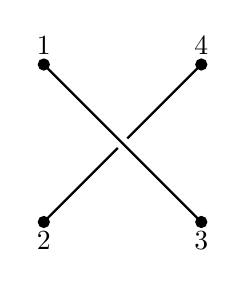
\begin{tikzpicture}
      \draw[black,thick] (-1,-1) -- (-.06,-.06);
      \draw[black,thick] (.06,.06) -- (1,1);
      \draw[black,thick] (-1,1) -- (1,-1);
      \filldraw[black] (-1,-1) circle (2pt) node[anchor=north] {2};
      \filldraw[black] (-1,1) circle (2pt) node[anchor=south] {1};
      \filldraw[black] (1,-1) circle (2pt) node[anchor=north] {3};
      \filldraw[black] (1,1) circle (2pt) node[anchor=south] {4};
    \end{tikzpicture}
  \end{center}
  \caption{Marginfigure: Tikz}
  \end{marginfigure}%
  \item \texttt{Margintable:} This environment requires the \texttt{$\backslash$begin\{margintable\}} {$\cdots$}\newline\texttt{$\backslash$end\{margintable\}} enclosings. A table package, such as \texttt{tabular}, \texttt{tabulary}, \texttt{tabu}, or \texttt{tabularx} is required. The \texttt{caption} package is needed to caption the table.
  \begin{margintable}
    \vspace{.1in}
    \begin{tabularx}{\marginparwidth}{|X|X|}
    \hline
    \textit{NotesTeX} & \textbf{rocks!}\\
    \hline
    \end{tabularx}
    \caption{Margintable}
  \end{margintable}
\end{enumerate}
\subsection{Why use both \texttt{marginnotes} and \texttt{sidenotes}?}
Quite simply, \texttt{marginnotes} overlap each other if they are too close. This means that figures, and tables can overlap by just using \texttt{marginnotes}. This is why \texttt{sidenotes} is so useful as it not only numbers all side notes, but also dynamically aligns all side notes, figures, and tables.

So clearly, \texttt{sidenotes} must be better right? There are a few places where \texttt{sidenotes} fails too however. For instance, \texttt{sidenotes} cannot be used in equations, \texttt{multicols}, and with the \texttt{tcolorbox}\sn{See \ref{Sub:Special} and \ref{Sec: Fullpage} for more details.} environment. As the majority of the special environments from \texttt{amsthm} are modified to use \texttt{tcolorbox}, \texttt{marginnotes} becomes an essential part of \textit{NotesTeX}.

\newpage

\section{\TeX\ Shortcuts}\label{sec:shortcuts}
\textit{NotesTeX} comes built in with a minimal set of keyboard shortcuts for a few special characters. All of these shortcuts can be found in \texttt{NotesTeX.sty} just under
\begin{verbatim}
% ----------------------------------------------------------------------
%           User Created Commands
% ----------------------------------------------------------------------
...
\end{verbatim}
If one has their own macros,\sidenote{\footnotesize Most people have their own shortcuts for commonly used mathematics, such as derivatives or integrals. For those looking for some physics shortcuts, the \textbf{supremely excellent} physics package (automatically included in \textit{NotesTeX}) has possible everything that one can imagine.} then simply add it under this area. 

\subsection{Available Shortcuts}
To keep things light, \textit{NotesTeX} offers the following simplifications/shortcuts to the mathematics dictionary.
\begin{enumerate}
  \item Vector Bold Math: The shortcut \texttt{\{$\backslash$bf $\cdot$\}} $\longrightarrow$ \texttt{$\backslash$bf$\cdot$} creates boldface text. For example, \texttt{\{$\backslash$bf a\}} becomes \texttt{$\backslash$bfa} producing the output \bfa. This works for both upper and lower case alphabet.
  \item \texttt{Mathfrak:} The \texttt{$\backslash$mathfrak} environment is quite similar to the Vector Bold Math in the shortcut argument, \texttt{$\backslash$mathfrak\{$\cdot$\}} $\longrightarrow$ \texttt{$\backslash$mf$\cdot$}. This works for both upper and lower case producing
  \begin{center}
    $\mfa\mfb\mfc\mfd\mfe\mff\mfg\mfh\mfi\mfj\mfk\mfl\mfm\mfn\mfo\mfp\mfq\mfr\mfs\mft\mfu\mfv\mfw\mfx\mfy\mfz$\\
    $\mfA\mfB\mfC\mfD\mfE\mfF\mfG\mfH\mfI\mfJ\mfK\mfL\mfM\mfN\mfO\mfP\mfQ\mfR\mfS\mfT\mfU\mfV\mfW\mfX\mfY\mfZ$
  \end{center}
  \item \texttt{Mathbb}: All \texttt{$\backslash$mathbb\{$\cdot$\}} objects are turned into \texttt{$\backslash$bb\{$\cdot$\}}. This only works for uppercase alphabet.
  \begin{equation*}
    \bbA\bbB\bbC\bbD\bbE\bbF\bbG\bbH\bbI\bbJ\bbK\bbL\bbM\bbN\bbO\bbP\bbQ\bbR\bbS\bbT\bbU\bbV\bbW\bbX\bbY\bbZ
  \end{equation*}
  \item \texttt{Mathcal:} All \texttt{$\backslash$mathcal\{$\cdot$\}} objects are turned into \texttt{$\backslash$mc\{$\cdot$\}}. This only works for uppercase alphabet.
  \begin{equation*}
    \mcA\mcB\mcC\mcD\mcE\mcF\mcG\mcH\mcI\mcJ\mcK\mcL\mcM\mcN\mcO\mcP\mcQ\mcR\mcS\mcT\mcU\mcV\mcW\mcX\mcY\mcZ
  \end{equation*}
\end{enumerate}


\newpage
\section{\texttt{amsthm} Environments}\label{Sub:Special}
\texttt{amsthm} environments are defined as usual being enclosed by \texttt{$\backslash$begin\{environment\}}$\cdots$ \texttt{$\backslash$end\{environment\}} and most have been modified ostensibly from the original \texttt{amsthm} presets. Primarily, most environments, with the exception of the exercise environment, are now integrated with the wonderful \texttt{tcolorbox} package. Note that the counting for \texttt{theorems} and \texttt{lemmas} is distinct from the counting for \texttt{definitions}. Also note that the \texttt{breakable} for \texttt{tcolorbox} allows these environments to span multiple pages.

\begin{definition}
  The \texttt{definition} environment and the associated \texttt{tcolorbox} are provided by the following code in \texttt{NotesTeX.sty}:
  \begin{verbatim}
    \tcolorboxenvironment{definition}{
      boxrule=0pt,
      boxsep=0pt,
      colback={White!90!Cerulean},
      enhanced jigsaw, 
      borderline west={2pt}{0pt}{Cerulean},
      sharp corners,
      before skip=10pt,
      after skip=10pt,
      breakable,
    }
  \end{verbatim}
\end{definition}
\begin{theorem}
  The \texttt{theorem} environment and the associated \texttt{tcolorbox} are provided by the following code in \texttt{NotesTeX.sty}:
  \begin{verbatim}
    \tcolorboxenvironment{theorem}{
      boxrule=0pt,
      boxsep=0pt,
      colback={White!90!Dandelion},
      enhanced jigsaw, 
      borderline west={2pt}{0pt}{Dandelion},
      sharp corners,
      before skip=10pt,
      after skip=10pt,
      breakable,
    }
  \end{verbatim}
\end{theorem}
\begin{lemma}
  The \texttt{lemma} environment and the associated \texttt{tcolorbox} are provided by the following code in \texttt{NotesTeX.sty}:
  \begin{verbatim}
  \tcolorboxenvironment{lemma}{
    boxrule=0pt,
    boxsep=0pt,
    blanker,
    borderline west={2pt}{0pt}{Red},
    before skip=10pt,
    after skip=10pt,
    sharp corners,
    left=12pt,
    right=12pt,
    breakable,
  }
  \end{verbatim}
\end{lemma}
\begin{proof}
  The \texttt{proof} environment and the associated \texttt{tcolorbox} are provided by the following code in \texttt{NotesTeX.sty}:
  \begin{verbatim}
    \tcolorboxenvironment{proof}{
      boxrule=0pt,
      boxsep=0pt,
      blanker,
      borderline west={2pt}{0pt}{NavyBlue!80!white},
      before skip=10pt,
      after skip=10pt,
      left=12pt,
      right=12pt,
      breakable,
    }
  \end{verbatim}
\end{proof}
\begin{example}
  The \texttt{example} environment and the associated \texttt{tcolorbox} are provided by the following code in \texttt{NotesTeX.sty}:
  \begin{verbatim}	
  \tcolorboxenvironment{example}{
    boxrule=0pt,
    boxsep=0pt,
    blanker,
    borderline west={2pt}{0pt}{Black},
    sharp corners,
    before skip=10pt,
    after skip=10pt,
    left=12pt,
    right=12pt,
    breakable,
  }
  \end{verbatim}
\end{example}	
\begin{remark}
  The \texttt{remark} environment and the associated \texttt{tcolorbox} are provided by the following code in \texttt{NotesTeX.sty}:
  \begin{verbatim}
  \tcolorboxenvironment{remark}{
    boxrule=0pt,
    boxsep=0pt,
    blanker,
    borderline west={2pt}{0pt}{Green},
    before skip=10pt,
    after skip=10pt,
    left=12pt,
    right=12pt,
    breakable,
  }
  \end{verbatim}
\end{remark}
\begin{exercise}
  The exercise environment remains unchanged from the \texttt{amsthm} presets.
\end{exercise}



\subsection{\texttt{tcolorbox} Environment and Known Issues} % (fold)
\label{ssub:tcolorbox environments_and_known_issues}

There is one issue with this however.\marginnote{Not a major one but frustrating nonetheless.} Since we are using a \texttt{tcolorbox}, this proof environment is incompatible with \texttt{$\backslash$sn} and \texttt{$\backslash$sidenote}, as it results in a \textbf{Float(s) Error}. However, this environment is compatible with \texttt{$\backslash$mn} and \texttt{$\backslash$marginnote} thankfully.\mn{As one can see right here.}


The \texttt{breakable} should allow the \texttt{proof} environment to span multiple pages. If one wishes to change the color, simply modify the line which states \texttt{borderline west=\{1pt\}\{0pt\}\{blue\}}. The first numeric value dictates the width of the line, the second dictates how close it is away from the \textit{left} margin, while the last argument obviously dictates the color. This code could also be used to change any of the other \texttt{amsthm} environments.

% subsubsection tcolorbox environments_and_known_issues (end)

\section{The Part Environment}\label{sec:part}
In the original Jhep format, the \texttt{$\backslash$part} environment is not special and is set to the default given by the article class. In \textit{NotesTeX}, the \texttt{part} environment produces the following image. Furthermore the code responsible is noted below.\\

\begin{fullpage}
{{\centering
  \begin{tcolorbox}[width=\marginparwidth,height=\marginparwidth/2,colback=black!75!white,colframe=black!75!white,center title,fonttitle=\bfseries\normalsize,title=PART,text fill]
    \begin{center}
    {\color{white}\Huge\bfseries\#}
    \end{center}
  \end{tcolorbox}
}}
~ \newline 
\begin{verbatim}
  \titleformat{\part}[hang]{{\thispagestyle{plain}}\Huge\bfseries}{\marginnote{
    \begin{tcolorbox}
    [width=\marginparwidth,height=\marginparwidth/2,colback=black!75!white,
       colframe=black!75!white,center title,fonttitle=\bfseries\normalsize,title=PART,
       text fill]

      \begin{center}
        {\color{white}\thepart}
      \end{center}

    \end{tcolorbox}
  }[-1.25in]}{0pt}{\Huge\bfseries}
\end{verbatim}
\end{fullpage}

This combines the \texttt{titlesec} and the \texttt{tcolorbox} packages, placing the title of the \texttt{$\backslash$part} on the left hand side, and the \texttt{$\backslash$part} number in the margin. It is recommended that one do not mess with this, other than changing the colors given by \texttt{colback} and \texttt{colframe}.
\newpage

\section{Fullpage Environment}\label{Sec: Fullpage}
\begin{fullpage}
  The \texttt{fullpage} environment is defined by
  \begin{center}
    \texttt{$\backslash$begin\{fullpage\}}\\
    $\cdots$\\
    \texttt{$\backslash$end\{fullpage\}}
  \end{center}
  with the with of the \texttt{fullpage} environment given by \texttt{$\backslash$textwidth}+\texttt{$\backslash$marginparsep}+\texttt{$\backslash$marginparwidth}.\\
\end{fullpage}
There are some clear benefits of having use of the full page at times. Suppose that one wants to place a figure that cannot fit into the margins, or if an equation is quite long and it bleeds into the margin, then the \texttt{fullpage} environment can both clearly separate these from the surrounding text and allot for the dimensions without hassle. The code in \texttt{NotesTeX.sty} that is responsible for the \texttt{fullpage} environment is given by\sn{This is also an example of why the \texttt{fullpage} environment is nice.}\\

\begin{fullpage}
    \begin{verbatim}
    \newenvironment{fullpage}{
    {\smallskip\noindent
    \begin{minipage}{\textwidth+\marginparwidth+\marginparsep}\hrule\smallskip\smallskip}
    {\smallskip\smallskip\hrule\end{minipage}\vspace{.1in}
    }
    \end{verbatim}
\end{fullpage}

\begin{remark}
  If one do not like the lines at the beginning and end of the \texttt{fullpage} environment, simply remove all the \texttt{$\backslash$hrule} that is in the code. Similarly, it is possible to change the vertical spacing after the \texttt{fullpage} is over, by modifying the \texttt{$\backslash$vspace\{\}} argument. 
\end{remark}

\begin{fullpage}
  \begin{multicols}{2}
  A major benefit of having a \texttt{fullpage} is the ability to use \texttt{multicols} to its fullest extent. For example, these empty sentences are an example of how effective the \texttt{multicols} package can be inside of the \texttt{fullpage} environment. 

  This would be especially useful for formatting exercises in multiple columns and it makes the text distinct from the rest of the \texttt{fullpage} environment. The author has run out of things to say.
  \end{multicols}
\end{fullpage}

\subsection{Known Issues with Fullpage}\label{Sub: Fullpage_Issues}

There are a few issues with the \texttt{fullpage} however. 
\begin{remark}
  Since the \texttt{fullpage} environment uses a \texttt{minipage}, and minipages do not work over multiple pages, one will need a new \texttt{fullpage} per page.	
\end{remark}
\begin{remark}
  \textbf{Also, please note \texttt{marginnote}, or \texttt{sidenotes} cannot be used in this environment.} Footnotes, on the other hand, can be used but are really ugly.
\end{remark}

\newpage

%	
	%\part{Advanced Page Formatting}
  %For those wanting to adjust the margin sizes, or the \texttt{fancyhdr} layout, there are a few comments that could be made here.
\section{Page Dimensions}
\textit{NotesTeX} relies on the \texttt{geometry} package to set its dimensions. The associated code is the deceptively simple chunk of code given by
\begin{verbatim}
  \geometry{paperheight=845pt,paperwidth=597pt,
        marginparsep=.02\paperwidth,marginparwidth=.23\paperwidth,
        hoffset=-1in, voffset=-1in, headheight=.02\paperheight,
        headsep=.03\paperheight,footskip=20pt,
        textheight=.84\paperheight,textwidth=.64\paperwidth}.
\end{verbatim}
Ignoring most of the arguments, the \texttt{$\backslash$paperheight} and \texttt{$\backslash$paperwidth} are set to be the standard $8\times11$ inches but in \texttt{pt} format instead. All other options, with the exception of \texttt{$\backslash$hoffset} and \texttt{$\backslash$voffset}, inherit fractions of \texttt{$\backslash$paperheight} and \texttt{$\backslash$paperwidth}, the most important being \texttt{$\backslash$marginparwidth}. Increasing \texttt{$\backslash$marginparwidth} causes the margin to bleed off of the right side of the page. In order to increase, one \textbf{must} decrease the \texttt{$\backslash$textwidth} accordingly.


\section{\texttt{Fancyhdr} Layout}
As mentioned before, \texttt{fancyhdr} is overridden on the title page, the contents page, and the \texttt{$\backslash$part} page, and sets the header for all other pages through the code
\begin{verbatim}
\pagestyle{fancy}%
\newlength{\offset}%
\setlength{\offset}{\marginparwidth + \marginparsep}%
\renewcommand{\sectionmark}[1]{\markboth{#1}{}}%
\renewcommand{\subsectionmark}[1]{\markright{#1}{}}%

\fancypagestyle{fancynotes}{%
  \fancyhf{}%
  \fancyheadoffset[rh]{\offset}%
  \renewcommand{\headrulewidth}{0pt}%
  \fancyhead[L]{\textsc{\leftmark}}%
  \fancyhead[R]{\footnotesize \textit{\rightmark}~~~~ \thepage}%
}%
\end{verbatim}
The header style is set so that it spans the width of the entire page as opposed to just the \texttt{$\backslash$textwidth} through the line \texttt{$\backslash$fancyheadoffset[rh]\{$\backslash$myoddoffset\}}. The \texttt{$\backslash$sectionmark} and \texttt{$\backslash$subsectionmark} are set up so that the \texttt{section} appears on the left and all \texttt{subsections} appear on the right along with the page number, and this is given in the last two lines of code.

%------------------------------------------------------------------------------
\end{document}
%==============================================================================